\section{Recurrent Neural Network}

\subsection{LSTM}

\begin{figure}[tbp]
\centering
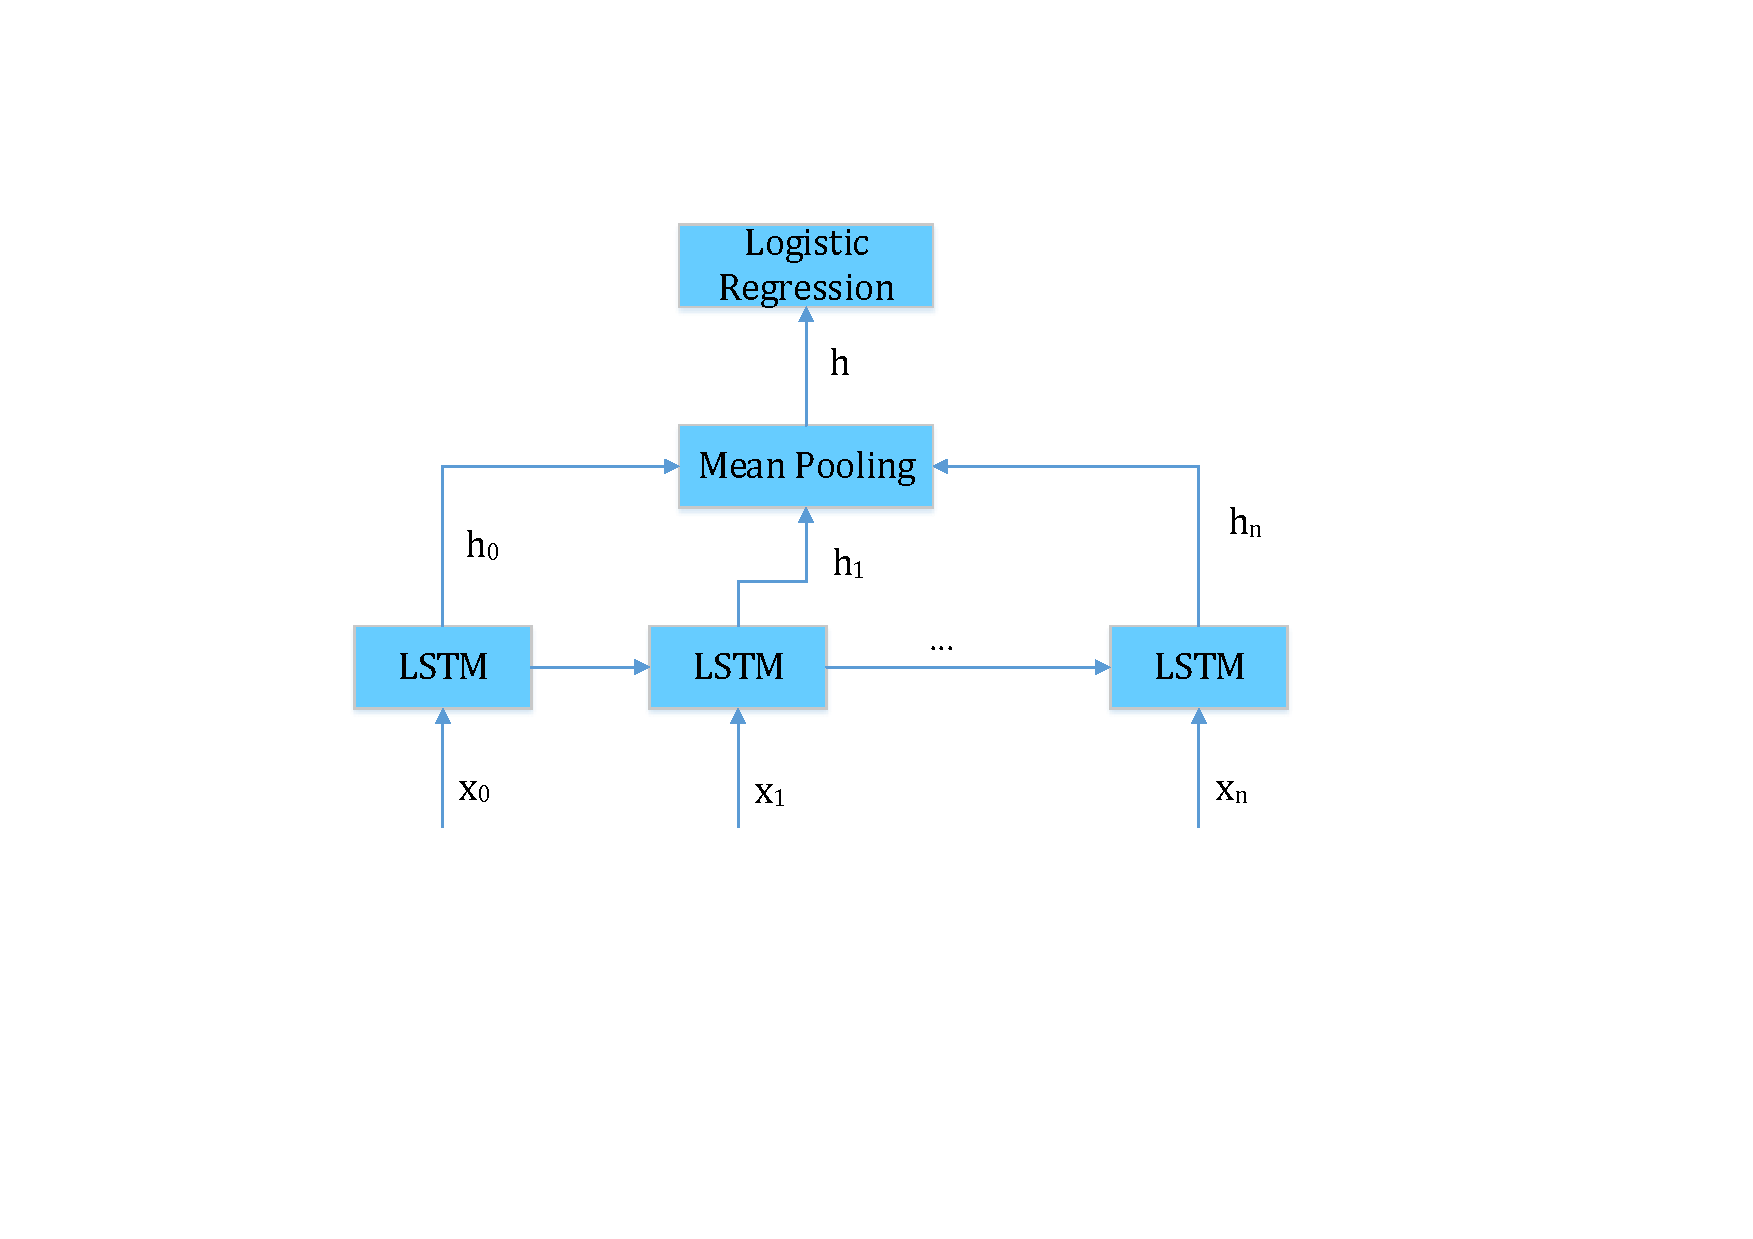
\includegraphics[scale=0.6]{figure/lstm_model.pdf}
\caption{LSTM model used in our report.}
\label{fig:lstm_model}
\end{figure}

For the LSTM model for sentiment analysis, we design and evaluate the model on two different kinds of sentiment data sets. The first one is the Stanford Twitter corpus, which has been described in previous section. And the second data set is the Large Movie Review Dataset~\cite{maas2011}, which consists of 25,000 highly polar movie reviews for training, and 25,000 reviews for testing. In the 25,000 training reviews, there are 12,500 positive reviews and 12,500 negative reviews.

During the pre-processing step, we utilize the count-based method to represent the words in the reviews. A count-based approach takes advantage of the assumption that words which have similar counts in a text context, share similar semantic meaning. This approach is opposite to context-predicting semantic vectors such as $word2vec$ which is used in our experiment of CNN. The difference between the two models were discussed in~cite{baroni2014}. 

The deep learning model we use in the report is a variance of classical LSTM. And the structure of the LSTM variance is shown in Figure~\ref{fig:lstm_model}. In our model, the output of current state does not depend on current memory cell state $C_t$, but just on input $x_t$ and $h_{t-1}$. So, the equation of $o_t$ is updated to
$$
o_t = \sigma (W_o x_t + U_o h_{t-1} + b_o)
$$

Additionally, the model also consists of a mean pooling layer and a logistic regression layer. For every LSTM cell, it outputs information $h_i$. And by averaging all of the output sequence, mean pooling outputs $h$ and it is fed to the logistic regression layer. Then the logistic regression layer will train the model according to class labels and associated sequences.

The LSTM model is implemented in Theano~\cite{bastien2012, bergstra2010}, which is a Python library for deep learning. It allows users to define, optimize and evaluate mathematical expression efficiently and conveniently. 
